	\documentclass[a4paper]{article}
	
	\usepackage[portuguese]{babel}
	\usepackage[utf8]{inputenc}
	\usepackage{indentfirst}
	\usepackage{graphicx}
	\usepackage{verbatim}
	\usepackage{wrapfig, blindtext}
	\usepackage{listings}
	\usepackage{textcomp}
	\usepackage{color}
	\usepackage{xcolor}
	\usepackage[left=1in,right=1in,top=1in,bottom=.8in]{geometry}
	\usepackage{float}

\graphicspath{ {res/} }

	%%%%%%%%%%% CONFIGURATION OF CODE INPUT %%%%%%%%%%%%%%%%%%%%%%
\lstset{
  language=C,
  tabsize=4,
  captionpos=b,
  numbers=left,
  frame=single,
  breaklines=true,
  rulecolor=\color{black},
  title=Struct linkLayer,
  commentstyle=\color{codeGreen},
  backgroundcolor=\color{codeBackground},
  numberstyle=\color{gray},
  keywordstyle=\color{blue} \textbf,%otherkeywords={xdata},
  keywords=[2]{xdata},
  keywordstyle=[2]\color{red}\textbf,
  identifierstyle=\color{black},
  stringstyle=\color{red}\ttfamily,
  basicstyle = \ttfamily \color{black} \footnotesize,
  showstringspaces=false ,
}
%%%%%%%%%%%%%%%%%%%%%%%%%%%%%%%%%%%%%%%%%%%%%%%%%%

	\begin{document}
	

\definecolor{codeBackground}{RGB}{220, 220, 220}
\definecolor{codeGreen}{RGB}{0, 150, 0}
	\setlength{\textwidth}{16cm}
	\setlength{\textheight}{22cm}
	
	\title{\Huge\textbf{Lab 2}\linebreak\linebreak\linebreak
	\Large\textbf{Relatório Final}\linebreak\linebreak
	\linebreak\linebreak
	
\includegraphics[scale=0.1]{./res/feup-logo.png}\linebreak\linebreak
	\linebreak\linebreak
	\Large{Mestrado Integrado em Engenharia Informática e Computação} \linebreak\linebreak
	\Large{Redes de Computadores}\linebreak
		}
	

	\author{
	\textbf{Grupo 3:}\\
	Francisco Rodrigues - 201305627 \\
	João Nogueira - up201303882 \\
	Marta Lopes - 201208067 \\
	\linebreak\linebreak \\
	 \\ Faculdade de Engenharia da Universidade do Porto \\ Rua Roberto Frias, s\/n, 4200-465 Porto, Portugal \linebreak\linebreak\linebreak
	\linebreak\linebreak\vspace{1cm}}
	
	\maketitle
	\thispagestyle{empty}

	\newpage

	\section{Introdução}
	\normalsize

Este relatório tem como objetivo explicar o segundo projeto da Unidade Curricular de Redes de Computadores bem como analisar os resultados obtidos na realização das experiências especificadas no enunciado do mesmo.

Este projeto encontra-se dividido em duas grandes partes. Em primeiro lugar, é-nos pedido que desenvolvamos uma aplicação de \textit{download} que proceda à transferência de um ficheiro e que implemente o protocolo \textit{FTP}. Em segundo lugar, é-nos pedido que configuremos e estudemos uma Rede de Computadores seguindo a estrutura das experiências abaixo enumeradas:

\begin{enumerate}

\item Configuração de um \textit{IP} de rede;
\item Configuração de duas Redes \textit{LAN} virtuais num \textit{switch};
\item Configuração de um \textit{router} em \textit{Linux};
\item Configuração de um \textit{router} comercial implementando \textit{NAT};
\item \textit{DNS};
\item Conexões \textit{TCP}.

\end{enumerate}

	\newpage

	\tableofcontents	

	\newpage

	\section{Parte 1 - Aplicação de download}

	Como referido anteriormente, a primeira parte deste tranalho consiste numa aplicação que transfere um ficheiro utilizando o protocolo \textit{FTP} descrito no ficheiro RFC959. Como método de \textit{input} é utilizada a sintaxe mostrada na figura abaixo como descrito no ficheiro RFC1738.

	\begin{figure}[H]
  	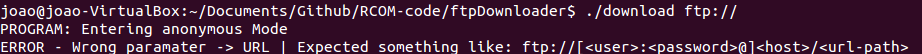
\includegraphics[width=\linewidth]{consoleScreenshot1.png}
  	\caption{Input}
  	\label{fig:input}
	\end{figure}

	A aplicação desenvolvida permite que seja feito um download em modo anónimo. Para tal basta não colocar os caracteres '@' e ':' e não colocar nome de utilizador e password. Neste caso a aplicação irá assumir o utilizador \textit{anonymous} e a palavra-passe vazia.

	\subsection{Arquitetura}

	A \textit{UrlStruct} é a estrutura definida respponsável por guardar a informação necessária que depende do \textit{input} do utilizador.

	\lstset{basicstyle=\ttfamily \color{black}\small, title=urlStruct}
	\lstinputlisting{./res/res1.c}
	\normalsize

	Ao correr o programa é chamada a função \textit{getUrlInfo} que é responsável por pegar na \textit{string} que o utilizador forneceu como argumento e interpretar toda a informação necessária.

	\lstset{basicstyle=\ttfamily \color{black}\small, title=Url Header}
	\lstinputlisting{../ftpDownloader/url.h}
	\normalsize

	\newpage

	\section{O Jogo - Q!nto}
	\subsection{História}
	
	“Q!nto” é um jogo de tabuleiro recente, criado no ano de 2014 no qual podem participar entre 2 e 4 jogadores. Foi criado por Gene Mackles e lançado pela PDG games
	
	Este jogo faz parte de uma coleção de três jogos chamada Triple Play que é uma coleção de jogos de tabuleiro.

	\subsection{Conteúdo do Jogo}
	
	Estão incluídas no Jogo 60 cartas divididas como mostra a figura à direita.
	
	\subsection{Regras de Jogo}
	
	Existem três versões para jogar o Q!into, sendo elas o
	\textit{Classic},
	\textit{Plus} e
	\textit{Light}. Neste projeto usaremos apenas a versão Light que passamos a explicar a seguir:
	
	Inicialmente cada jogador retira uma carta do baralho para escolher quem começa a jogar. O jogo começa dividindo igualmente o baralho pelos jogadores presentes.
	
	As cartas que cada jogador recebeu serão a pilha de cartas com que ele vai poder jogar. Estas ficarão viradas para baixo e cada jogador retira da pilha de cartas que lhe foi atribuída as primeiras 5. 
	
	\textbf{Noção base:} Uma linha são 2, 3, 4 ou 5 cartas numa linha ou coluna na qual as cartas têm a mesma côr ou cores diferentes e na qual as cartas têm a mesma forma ou formas diferentes. Uma linha com 5 cartas é um Q!nto.
	O primeiro jogador começa o jogo. A seguir joga o jogador à sua esquerda. Quando na vez de um jogador, este pode fazer uma de três coisas:
	
	\begin{enumerate}
	\item 		Adicionar 1, 2, 3, 4 ou 5 peças à grelha numa única linha reta e depois retirar do topo da sua pilha de cartas o número necesário para voltar a ficar com 5 na mão*.
	Se, numa das jogadas, o jogador completar um ou mais Q!ntos, este deve voltar a completar a sua mão* e deve jogar outra vez.
	\item		Trocar uma ou mais cartas da sua mão por wildcards já jogadas e/ou a carta Q!nto de forma a que as cartas trocadas continuem a funcionar naquela posição.
	\item		Passar a vez... e trocar algumas, todas ou nenhuma das susas cartas colocando-as no fundo da sua pilha e retirando do topo o número de cartas necessário para voltar a ficar com 5*.
	\end{enumerate}
	
	\small
	*ou menos, se não houver cartas suficientes para perfazer 5.
	\normalsize
	
	\bigskip
	
	O jogo termina quando houver 1 jogador que fica sem cartas, sendo este o vencedor.\newline
	
	\small
	\noindent
	Nota: Uma carta “wild” ou “Q!nto” pode representar cartas diferentes em diferentes direções. No caso de representar coisas diferentes e não ter na mão uma carta que também as consiga representar, então, essa carta é insubstituível.
	\normalsize
	\newpage

	\section{Lógica de Jogo}
	\subsection{Representação do estado de jogo}

	Embora não haja tabuleiro neste jogo, existe sempre a necessidade de saber a posição relativa entre as cartas que estão em jogo. Como tal, implementamos um tabuleiro na forma de lista de listas de cartas que funciona de forma dinâmica, ou seja, sempre que é introduzida uma nova carta é feita a verificação aos quatro lados do tabuleiro e adicionada uma linha/coluna se assim for necessário, por forma a garantir que existem sempre casas nas bordas do tabuleiro que estão livres para que o jogador as possa utilizar.
	
O estado do jogo não é apenas representado pelo tabuleiro. A cada jogada é apresentada no ecrã a mão de que o jogador dispõe para jogar. Como sabemos ele apenas tem acesso a cinco das cartas do seu baralho, e durante a sua jogada não lhe são dadas mais cartas para além daquelas cinco.
	
	\subsection{Visualização do Tabuleiro}

	Sendo o tabuleiro uma lista de listas de tamanho variável, os predicados responsáveis pela visualização do tabuleiro de jogo terminam quando a cauda da lista é uma lista vazia nas chamadas recursivas como mostrado abaixo.

	Alguns dos predicados utilizados não estão mostrados acima, como por exemplo o predicado responsável pela impressão dos índices das linhas, no entanto estes estão incluídos no código fonte em anexo a este relatório.

	\subsection{Execução de Jogadas}

	No início de cada jogada é perguntado ao jogador que tipo de jogada pretende executar. Como sabemos acima o jogador pode optar por adicionar cartas, trocar cartas já presentes no tabuleiro ou trocar cartas que tem na mão.

	\subsubsection{Adicionar Cartas}

	Depois de optar por adicionar cartas no tabuleiro, é mostrado no ecrã o estado atual do tabuleiro e as cartas que o jogador tem na mão. O jogador opta pelas cartas que quer jogar bem como a casa do tabuleiro onde pretende que as cartas sejam colocadas. Depois de introduzir esses dados é feita a verificação das condições que têm de ser cumpridas:

	\begin{itemize}
		\item 	Verifica se a casa está vazia;
		\item Verifica se tem pelo menos uma carta nas casas adjacentes (excepto no caso de ser a primeira jogada);
		\item Verifica se, com a carta colocada, a linha fica com menos de seis cartas;
		\item Verifica também se as regras relacionadas com as cores e naipes se verificam na linha;
		\item Verifica se, com a carta colocada, a coluna fica com menos de seis cartas;
		\item Verifica também se as regras relacionadas com as cores e naipes se verificam na coluna.
	\end{itemize}

	Acima encontra-se parte do predicado responsável pelas verificações mencionadas que garantem que todas as regras são cumpridas.

	\subsubsection{Trocar Cartas}

	Depois de optar por alterar cartas presentes no tabuleiro, tal como no caso acima, é mostrado no ecrã o estado atual do tabuleiro bem como as cartas de que o jogador dispõe. Depois de optar pelas cartas e casas nas quais querem jogar são feitas as seguintes verificações:

	\begin{itemize}
		\item Verifica se a carta escolhida pelo jogador é \textit{Wild}, seja de côr ou naipe;
		\item Verifica se a casa escolhida pelo utilizador está, de facto, ocupada;
		\item Verifica se as regras referentes ao número, cores e naipes da sequência são cumpridas na linha;
		\item Verifica se as regras referentes ao número, cores e naipes da sequência são cumpridas na coluna.
	\end{itemize}

	Acima encontra-se parte do predicado responsável pelas verificações mencionadas que garantem que todas as regras são cumpridas.

	\subsubsection{Trocar cartas}

	Ao optar por trocar cartas é dada oportunidade ao jogador para escolher quais as cartas (dentro daquelas que estão nesse momento na sua mão) que este pretende trocar. Após a escolha estas cartas passam para o fim do baralho e são repostas na mão por aquelas que estão imediatamente no topo do baralho.

	\subsection{Avaliação do estado do Jogo}

	Tendo em conta que nesta modalidade o jogo termina quando um dos jogadores termina o seu baralho, podemos avaliar o estado do jogo através do número de cartas restantes nos baralhos dos jogadores que são impressos nas jogadas.

	\subsection{Final do Jogo}

	O jogo termina mal um dos jogadores termine com o seu baralho, tendo sido bem sucedido em deixar todas as suas cartas no tabuleiro sem infringir nenhuma das regras. No final de cada jogada é feita a verificação de se o baralho do jogador está, ou não, vazia. No caso do baralho estar vazio termina o jogo imediatamente.

	\newpage

	\section{Interface com o Utilizador}

	\clearpage

	\section{Conclusões}

	Este trabalho realizado no âmbito da Unidade Curricular de Programação em Lógica serviu positivamente para que ganhássemos bastantes conhecimentos ao nível da linguagem de PROLOG. Achamos que, tendo um pouco mais de tempo para a conclusão do trabalho, este seria concluído de melhor forma. Mesmo assim o balanço que fazemos é bastante positivo.

	Surpreendeu-nos a dificuldade de algumas das regras exigidas por este jogo, bem como a necessidade de fazer um tabuleiro de forma dinâmica, no entanto, encaramos estas dificuldades como desafios que fizemos por superar e fizemo-lo com sucesso. Infelizmente não tivemos tempo para implementar o \textit{bot}, melhoria que proporíamos num futuro em que pudéssemos melhorá-lo.

	%************************************************************************************************


	\end{document}
